% Please give the surname of the lead author for the running footer
\leadauthor{Tosheva \& Laine}

% info about NM-BC format: https://www.nature.com/nmeth/about/content

\title{NanoJ: a high-performance open-source super-resolution microscopy toolbox}
%NM-BC: The title is limited to 10 words (or 90 characters)
\shorttitle{NanoJ}

% Use letters for affiliations, numbers to show equal authorship (if applicable) and to indicate the corresponding author
\author[1,2\space *]{Kalina L. Tosheva}
\author[1-3\space *]{Romain F. Laine}
\author[1,2,4]{Nils Gustafsson}
\author[1,2,4]{Robert D. M. Gray}
\author[1,2]{Pedro Almada}
\author[1]{David Albrecht}
\author[1,6]{Gabriel Tarrason Risa}
\author[7]{Ann-Christin Lindås}
\author[1,6]{Buzz Baum}
\author[1]{Jason Mercer}
\author[5]{Christophe Leterrier}
\author[1-3\space\Letter]{Pedro M. Pereira}
\author[1-3\space\Letter]{Si\^{a}n Culley}
\author[1-3\space\Letter]{Ricardo Henriques}

\affil[1]{MRC-Laboratory for Molecular Cell Biology. University College London, London, UK}
\affil[2]{Department of Cell and Developmental Biology, University College London, London, UK}
\affil[3]{The Francis Crick Institute, London, UK}
\affil[4]{Centre for Mathematics and Physics in Life Sciences and Experimental Biology (CoMPLEX), University College London, London, UK}
\affil[5]{Aix-Marseille Univ, CNRS, INP, Inst Neurophysiopathol, NeuroCyto, Marseille, France}
\affil[6]{Institute for the Physics of Living Systems, University College London, London, UK}
\affil[7]{Department of Molecular Biosciences, The Wenner-Gren Institute, Stockholm University, Stockholm, Sweden}

\affil[*]{These authors contributed equally.}

\maketitle

%TC:break Abstract
\begin{abstract}
%Lets try to keep the abstract between 70-150 words, I have noticed no guidance

Super-resolution microscopy has become essential for the study of nanoscale biological processes. This type of imaging often implies the use of specialised image analysis tools to process a large volume of recorded data and extract quantitative information. In recent years, our team has built an open-source image analysis framework for super-resolution microscopy designed to combine for high performance and ease of use. We named it NanoJ - a reference to the popular ImageJ software it was developed for. In this paper, we highlight the current capabilities of NanoJ for several essential processing steps: spatiotemporal alignment of raw data (NanoJ-Core), super-resolution image reconstruction (NanoJ-SRRF), image quality assessment (NanoJ-SQUIRREL), structural modelling (NanoJ-VirusMapper) and control of the sample environment (NanoJ-Fluidics). We are constantly expanding NanoJ with the aim of improving quantitative analysis and thus foster the reliability of biological microscopy studies.

\end {abstract}
%TC:break main
%the command above serves to have a word count for the abstract

\begin{keywords}
    ImageJ | Fiji | super-resolution microscopy | Image analysis | Fluidics | Resolution | Quantitative imaging | Modelling
\end{keywords}

\begin{corrauthor}
    p.pereira\at ucl.ac.uk, s.culley\at ucl.ac.uk, r.henriques\at ucl.ac.uk
\end{corrauthor}

%%%%%%%%%%%%%%%%
% Introduction %
%%%%%%%%%%%%%%%%
% ------------------------------------------------------------------------------------------------------------------------------------

\subsection*{Introduction}
Fluorescence microscopy has been ubiquitously used in biological studies since its invention in the 20\textsuperscript{th} century. It can reveal subcellular structures and interactions between specifically labelled molecules, and allows the quantification of their dynamic behaviour in living cells \cite{rino2009frontiers}. Extraction of this biologically relevant quantitative information from fluorescence microscopy data typically requires digital image processing and analysis \cite{wheeler2017standard}. In recent years, Super-Resolution Microscopy (SRM) techniques \cite{betzig2006imaging,rust2006sub,hell1994breaking} have extended the spatial resolving power of fluorescence microscopy beyond that of the diffraction limit. Most SRM techniques use large quantities of raw data, often reaching several gigabytes for a single image, and thus require specialised high-performance image analysis tools.  Several SRM image processing packages are available, such as ThunderSTORM \cite{ovesny2014thunderstorm}, LAMA \cite{Malkusch2016LAMA} and SIMcheck \cite{schermelleh2015simcheck}, but each of these is focused on a specific type of SRM modality.
  
 %TC:ignore
 \begin{figure}[!t]
    \centering
    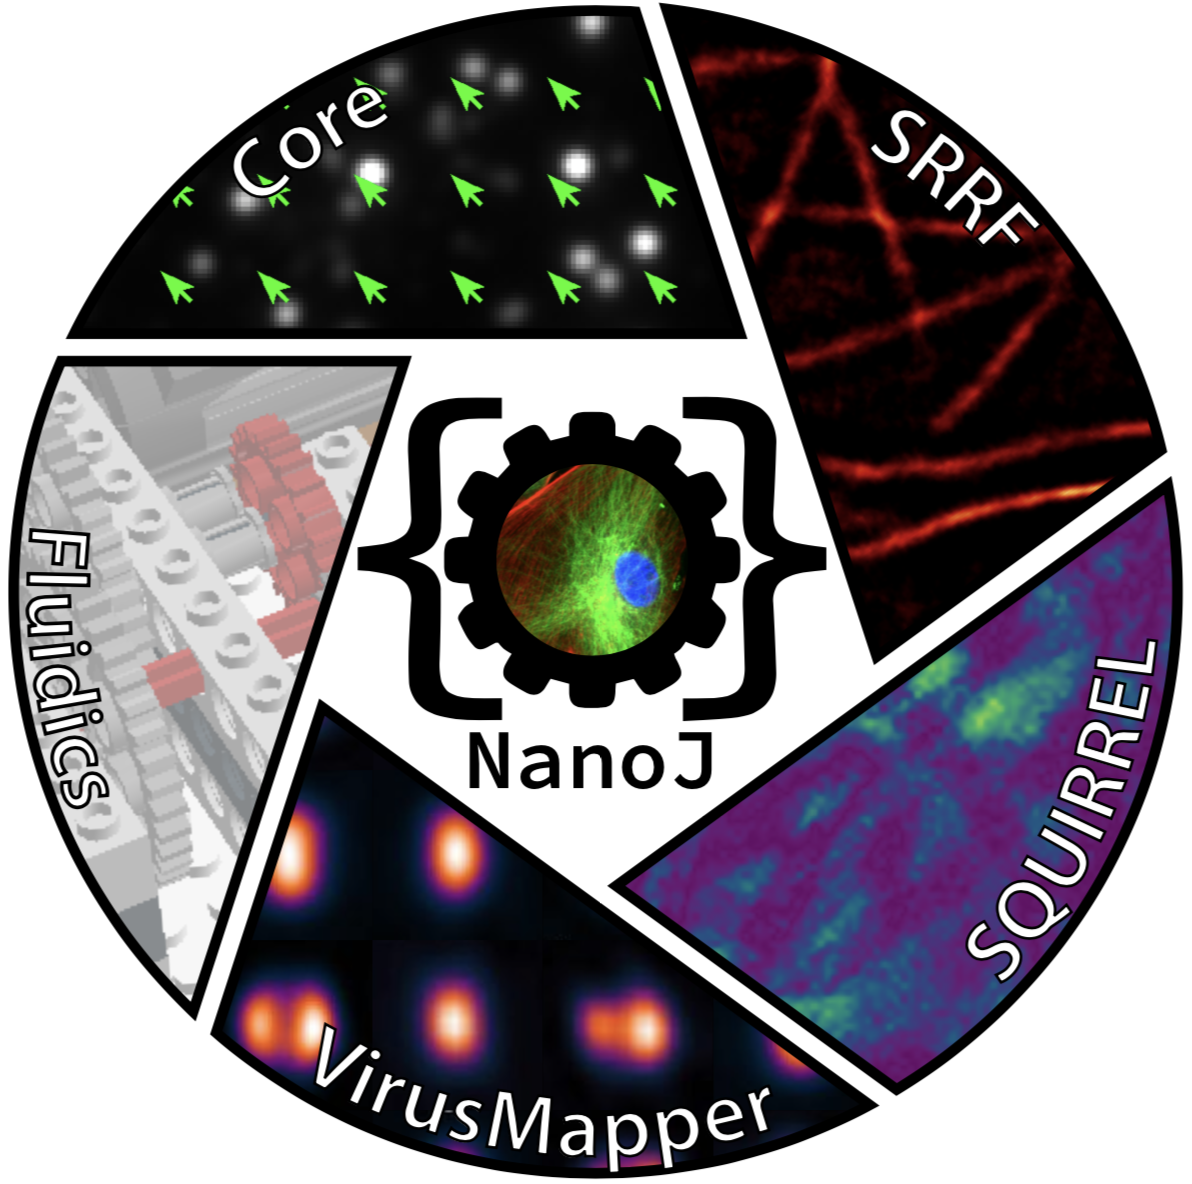
\includegraphics[width=\linewidth]{Figures/FigureMain_v3.png}
    \caption{\textbf{NanoJ framework.} Currently NanoJ consists of 5 modules dedicated to super-resolution imaging and analysis.}
    \label{fig:GeneralDiagram}
 \end{figure}
 %TC:endignore
 
%  linewidth: \printinunitsof{in}\prntlen{\linewidth}

 Here, we present NanoJ, a highly versatile set of image acquisition and analysis methods developed to improve microscopy experiments, with a particular focus on the demands of live-cell SRM. NanoJ is available as a series of ImageJ-based plugins which can be used independently or concomitantly to obtain high-fidelity images from which qualitative and quantitative information can be extracted. NanoJ is comprised of (Fig. \ref{fig:GeneralDiagram}): \textbf{NanoJ-Core} - general image correction tools including drift correction and channel registration, both based on cross-correlation analysis; \textbf{NanoJ-SRRF} - an analytic approach capable of extracting super-resolution data from a short burst sequence of diffraction-limited images, which can be acquired using most microscopes \cite{gustafsson2016fast,culley2018srrf}; \textbf{NanoJ-SQUIRREL} - an algorithm to evaluate resolution and the presence of artefacts in super-resolution images \cite{culley2018quantitative}; \textbf{NanoJ-VirusMapper} - a single-particle analysis method to generate nanoscale models of repetitive meta-stable biological structures such as viruses \cite{gray2016virusmapper,gray2017open,gray2018nanoscale}; \textbf{NanoJ-Fluidics} - a software interface to control fluidic hardware devices, enabling automation, e.g. of multiplexed experiments \cite{almada2018automating}. Thus the NanoJ framework is capable of solving common imaging problems with broad biological applications, and is compatible with a multitude of fluorescence microscope setups and experimental protocols. 
 
\subsection*{The NanoJ framework}
 NanoJ has been designed to integrate with the popular ImageJ or Fiji image analysis software \cite{abramoff2004image,schindelin2012fiji}, and is easily installed as a standard set of plugins. While the methods within NanoJ make use of state-of-the-art high-performance computing, NanoJ is also fully open-source and user-friendly. The graphical user interfaces (GUIs) are straightforward to use and its routines can be easily integrated within larger image analysis pipelines through the ImageJ macro language.

 NanoJ comprises several modules, each with their own separate manual and documentation. It is designed to be an accessible tool for both non-expert users and developers. NanoJ is implemented in both Java (\href{https://www.java.com/}{https://www.java.com/}) and OpenCL (\href{https://www.khronos.org/opencl}{https://www.khronos.org/opencl}), the latter language being used for high-performance analysis of image data through the use of Graphical Processing Units (GPUs). To date, it encompasses four Java ARchive (JAR) packages (NanoJ-SRRF, NanoJ-SQUIRREL, NanoJ-VirusMapper, NanoJ-Fluidics) that all depend on a central package (NanoJ-Core). The core package hosts the libraries that enable high-performance GPU-based computing analysis and a set of basic image analysis helper methods. The modular nature of NanoJ means that its components can be updated independently and the framework can be easily extended by appending new analytic packages.

\subsection*{NanoJ-Core: Drift Correction}
Sample drift commonly occurs during the acquisition of SRM data, often as a result of gradual changes in the temperature of microscope components. Drift introduces motion blur artefacts and thereby a loss of resolution. While most modern microscopes have an active focus-lock device that stabilises the motion of the sample in the axial direction (minimizing focal drift), the sample will still be prone to lateral movement (Fig. \ref{fig:DriftCorrection}a). However, in the case where the raw data is made up of a sequence of consecutive frames acquired rapidly, as is common in SRM methods such as Single Molecule Localization Microscopy (SMLM) \cite{betzig2006imaging,rust2006sub} or fluctuation-based approaches \cite{gustafsson2016fast,dertinger2009fast,cox2012bayesian}, this lateral drift can be estimated (Fig. \ref{fig:DriftCorrection}b) and analytically corrected via post-processing (Fig. \ref{fig:DriftCorrection}c-d).
 
  %TC:ignore
 \begin{figure}[!t]
    \centering
    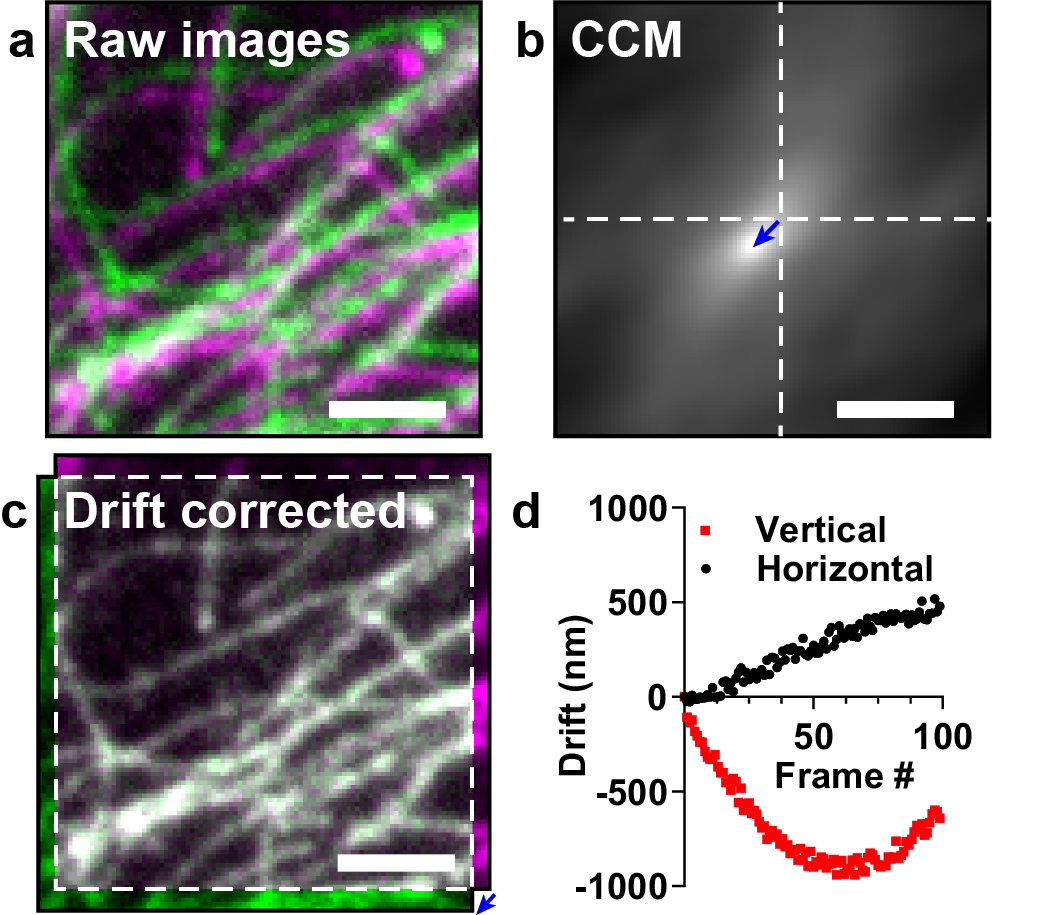
\includegraphics[width=\linewidth]{Figures/FigureDrift_v2.png}
    \caption{\textbf{Drift correction with NanoJ-Core.} \textbf{a)} Composite image of two frames of the same field-of-view with computationally-added visible drift. \textbf{b)} Cross-correlation map between the two frames shown in a). The vector position of the maximum indicates the linear shift between the two frames. \textbf{c)} Overlay of the two frames after drift correction using NanoJ-Core. \textbf{d)} Example vertical and horizontal drift curves obtained from 100 consecutive frames.}
    \label{fig:DriftCorrection}
 \end{figure}
 %TC:endignore

 NanoJ breaks the task of drift correction into two distinct parts: estimation, followed by translation. As a first step NanoJ-Core estimates the linear drift between two images by calculating their cross-correlation matrix (CCM) (Fig. \ref{fig:DriftCorrection}b). The location of the peak intensity in the CCM determines the linear shift between the two images, and precise sub-pixel accuracy is achieved by up-scaling the CCM using a bicubic spline interpolation. Depending on the type of acquisition, the reference frame can either be the first frame of the raw data (e.g. for a fixed sample) or the immediately preceding frame (for a live sample). Fig. \ref{fig:DriftCorrection}d shows the drift in a 100-frame dataset as measured with respect to the first frame. Once drift is estimated, the dataset can be directly corrected by analytically translating each individual frame using a bicubic spline interpolation (Fig. \ref{fig:DriftCorrection}c). The interpolation process will however change the noise properties of the resulting dataset \cite{blaysat2016effect}.
 
 For the specific case of SMLM datasets with sparse blinking, there will only be a weak correlation across frames, as there is little observable structure conserved between consecutive time points. One common strategy to alleviate this low correlation is to add fiduciary landmarks to the sample, such as static fluorescent beads. Alternatively, NanoJ-Core can temporally bin images within the dataset thus increasing the correlation between binned frames and allowing their shift to be more accurately estimated \cite{mlodzianoski2011sample}. 

 Drift estimation in NanoJ differs from strategies applied by other SRM algorithms, such as ThunderSTORM \cite{ovesny2014thunderstorm}, by analysing unprocessed raw data instead of post-processed Super-Resolution reconstructions. This allows the estimation to be decoupled from the Super-Resolution image reconstruction algorithm, and hence drift-corrected raw data can be analysed using a wider range of methods including SRRF and SOFI \cite{dertinger2009fast}. Furthermore, NanoJ-SRRF can import the created drift-table and use this information directly during analysis without the need to pre-translate each frame in the raw dataset.

\subsection*{NanoJ-Core: Channel registration}

In multicolour fluorescence microscopy, images acquired in different spectral channels are misaligned as a result of chromatic aberrations in the optical path and the use of different filter sets for each colour. This misalignment is frequently ignored in conventional microscopy as it typically occurs on a scale smaller than the diffraction limit; however, this effect becomes non-negligible in the context of SRM \cite{erdelyi2013correcting}. Correcting for spectral misalignment is essential for multicolour SRM studies quantifying colocalisation or interactions between different structures \cite{bock2007two,van2009multicolor,niekamp2017high}. 
 
 The shift between different spectral channels is usually inhomogeneous across a field of view, which prevents the use of typical CCM-based approaches such as the one described above in NanoJ-Core Drift Correction. In order to characterise the spectral misalignment across a field of view, it is necessary to image a sample that has the same structure present across several different wavelengths. Furthermore, the sample should contain structures occupying the whole field of view. A typical sample for this characterisation is a coverslip coated with a large number of beads labelled with multiple different dyes \cite{Demmerle2017}. Following multicolour imaging of this sample, NanoJ-Core can be used to calculate a non-linear two-dimensional spatial transform describing the misalignment for each channel relative to a 'reference' channel (Fig. \ref{fig:ChannelAlignment}a). NanoJ-Core can then apply these transforms to realign other multicolour datasets acquired using the same optical path (Fig. \ref{fig:ChannelAlignment}b) \cite{arganda2006consistent,annibale2012identification}. 
 
 To generate these non-linear misalignment fields NanoJ-Core first calculates local, quasi-linear misalignments between channels. This is achieved by dividing the image into small areas ('blocks'). For each block, the shift between the channel to be realigned and the reference channel is calculated by finding the cross-correlation peak position as shown in Fig. \ref{fig:DriftCorrection}a-b. These local shift values are then  interpolated across the whole field-of-view using an inverse distance weighting interpolation \cite{shepard1968two}. This generates two smooth 'shift' maps describing the misalignments in the horizontal and vertical directions (Fig. \ref{fig:ChannelAlignment}b). For a given channel, each pixel value within the horizontal/vertical shift map indicates the horizontal/vertical displacement that needs to be applied to that pixel to align it with the reference channel. NanoJ-Core can then be used to apply these maps to align channels in the original dataset (e.g. Fig. \ref{fig:ChannelAlignment}a, 'After registration'), or other datasets, provided they have been acquired using the same optical configuration.
 
 \begin{figure}[!t]
    \centering
    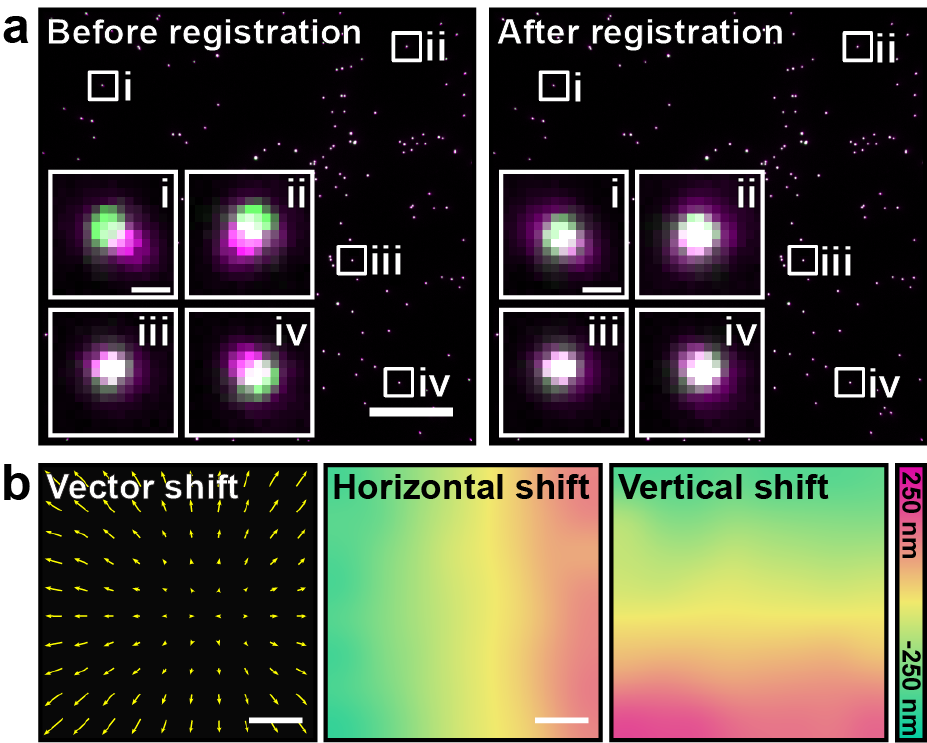
\includegraphics[width=\linewidth]{Figures/FigureChannelAlignment_v4.png}
    \caption{\textbf{Multi-colour channel registration with NanoJ-Core.} \textbf{a)} Composite image of multi-colour TetraSpeck beads imaged in two different channels (GFP channel indicated in green and mCherry channel in magenta), prior to (left) and after (right) channel registration using NanoJ-Core, acquired on a Nikon Ti2 frame with the CFI Apochromat TIRF 100XC Oil objective. Insets - individual beads from indicated locations, 1.63 x 1.63 \micro m. Scale bars: 25 \micro m. \textbf{b)} Horizontal and vertical shift maps obtained and applied to the data shown in a). Scale bars: 25 \micro m.}
    \label{fig:ChannelAlignment}
\end{figure}
 
 NanoJ-Core performs the channel registration by creating a new image representing each channel, where the intensity value for each pixel coordinate corresponds to the intensity value from the original image at the equivalent coordinate corrected for local shift. For cases in which these coordinates are not discrete (sub-pixel shift), a bicubic spline interpolation is used to recover pixel values in continuous space. Because the shift map can be extrapolated to continuous space, the registration procedure obtained from diffraction-limited images can also easily be used to correct super-resolved images obtained using the same optical configuration.
 
\subsection*{NanoJ-SRRF: Live-Cell Super-Resolution Imaging}

 As part of the NanoJ framework, we include our recently developed SRM reconstruction algorithm Super-Resolution Radial Fluctuations (SRRF), which is able to extract sub-diffraction information from a short burst of images acquired at high-speed with modern fluorescence microscopes \cite{gustafsson2016fast,culley2018srrf}. SRRF is a purely analytical approach. It alleviates the need to use toxic photoswitching-inducing buffers \cite{henriques2011palm}, specialised fluorophores \cite{dempsey2011evaluation,henriques2009palm}, damaging high-intensity illumination \cite{waldchen2015light} or specialised equipment \cite{gustafsson2000surpassing,hell1994breaking} when compared to other SRM methods \cite{betzig2006imaging,rust2006sub,gustafsson2000surpassing,hell1994breaking}.
 
 %TC:ignore
 \begin{figure}[!t]
    \centering
    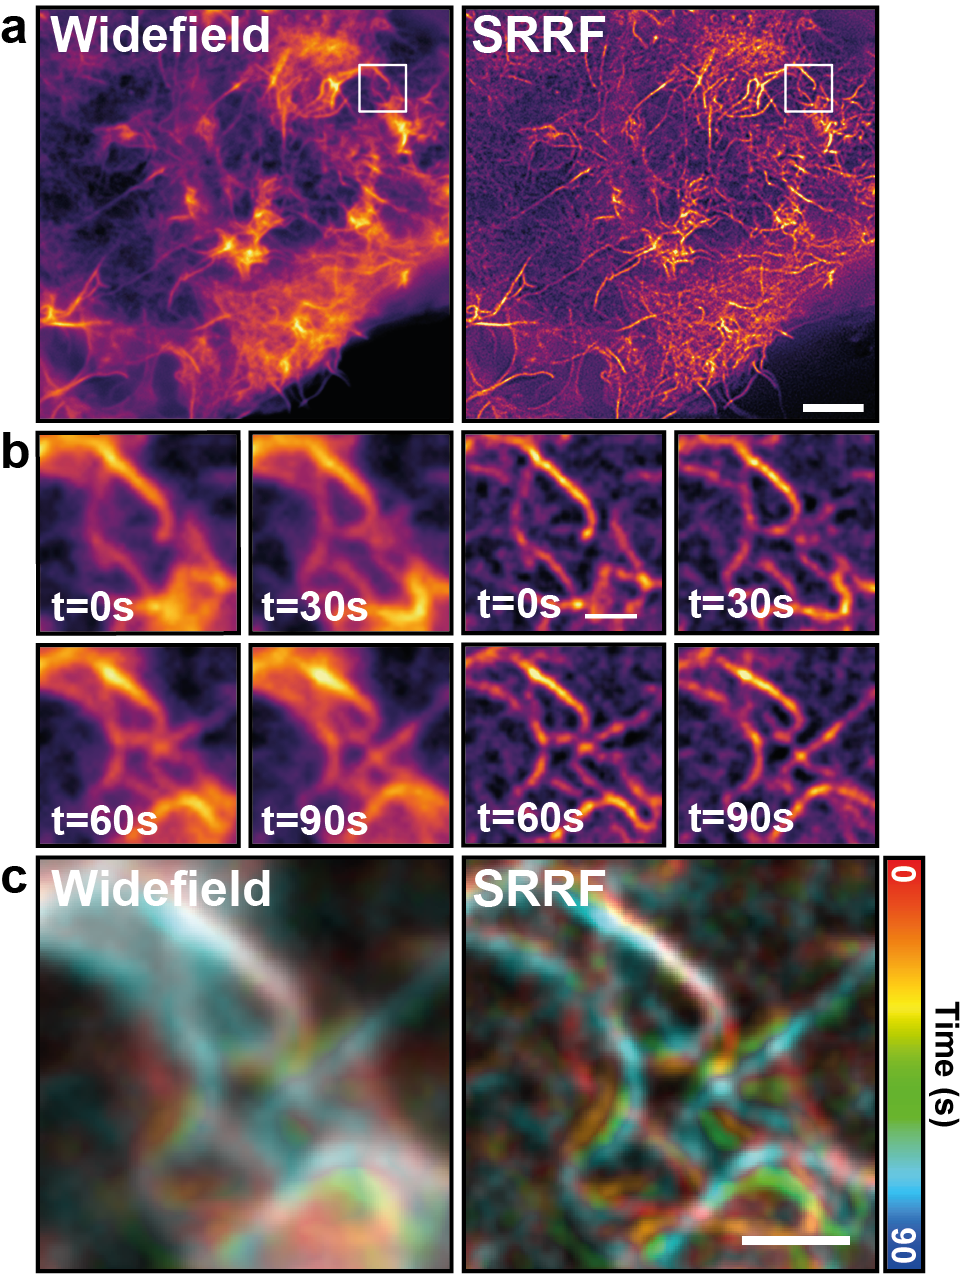
\includegraphics{Figures/FigureSRRF_v5.png}
    \caption{\textbf{Live-cell super-resolution with NanoJ-SRRF.} \textbf{a)} Comparison of widefield (left) and SRRF reconstruction (right) obtained from a Cos7 cell expressing UtrCH-GFP to label actin filaments. Scale bar: 5 \micro m. \textbf{b)} Time-course of the inset shown in a), obtained from  a continuous imaging at 30 ms exposure (33.3 Hz) and displayed every 30 s. Scale bar: 1 \micro m. \textbf{c)} Colour-coded time course dataset from b). Scale bar: 1 \micro m.}
    \label{fig:SRRF}
 \end{figure}
 %TC:endignore
 
 SRRF is based on similar principles to SMLM, however with the key difference that it does not rely on the detection of spatio-temporally isolated fluorophores. Instead, SRRF generates a magnified pixel grid where each pixel value relates to the probability of fluorophores existing in that corresponding region of space. To do this, SRRF calculates the local radial symmetry ('radiality') in each pixel of the magnified image using local intensity gradient information. The obtained radiality value will be high when a point-spread-function (PSF) profile transiently becomes dominant, highlighting the presence of a fluorescent molecule at that location. Furthermore, the fluctuations of radiality values follow the underlying natural intensity fluctuations of fluorophores, which have a distinct temporal signature to that of noise \cite{dertinger2009fast}. A temporal correlation of the radiality at each pixel can then be projected into a final image, where the structures of interest can be better resolved (Fig. \ref{fig:SRRF}).

 Thanks to its low-light requirement, SRRF is highly suited for live-cell SRM and allows for long SRM time-lapse acquisitions \cite{culley2018srrf}. Fig. \ref{fig:SRRF}a-c shows a typical live-cell SRRF acquisition of a Cos7 cell expressing UtrCH-GFP (a probe for actin filaments) imaged at 33.3 Hz for > 30 min. SRRF allows the observation of protein dynamics (e.g. actin) during long periods with no perceivable phototoxicity. 
 
 NanoJ-SRRF, the software implementation of the SRRF algorithm, uses GPU computing whenever possible to accelerate the radial symmetry calculations. This is achieved by implementing a large set of the required calculations in OpenCL, with a fallback of execution to the CPU if a compatible graphics card is not detected. NanoJ-SRRF can use a drift-table as an additional input, dynamically using its values to compensate for unwanted sample drift during the calculation of radial symmetries and temporal correlations.

\subsection*{NanoJ-SQUIRREL: Estimating Image Quality}
SRM techniques are more complex than conventional diffraction-limited microscopy. This complexity arises from the sample preparation requirements (SMLM), the microscope hardware (STED, SIM), and the post-acquisition image processing (SMLM, SIM). Unsuitable choices in any of these underlying variables can lead to artefacts within the final image and the potential for false conclusions to be drawn. NanoJ-SQUIRREL (Super-resolution Quantitative Image Rating and Reporting of Error Locations) is an algorithm that highlights the presence of artefacts in super-resolution images. It does so by calculating quantitative maps showing both local SRM image quality and resolution \cite{culley2018quantitative}, and can thus be used to optimise acquisition workflows \cite{culley2018srrf}.

 The central concept of SQUIRREL is that a diffraction-limited image and the corresponding SRM image of the same region should contain the same underlying structure, just at different resolutions. Thus the diffraction-limited image can be treated as a high-confidence benchmark against which the SRM image can be compared. The SQUIRREL image quality assessment algorithm formalises this comparison analytically.

NanoJ-SQUIRREL quality assessment requires the user to provide an acquired diffraction-limited `reference’ image and SRM image of the same structure (Fig. \ref{fig:SQUIRREL}a). As both images represent the underlying fluorophore distribution but at different resolutions, there exists a blurring function that can convert the SRM image into its diffraction-limited equivalent. SQUIRREL calculates this blurring function and applies it to the SRM image. The blurred image is then compared against the reference. This generates three quality indicators. An `error map’ is produced that maps the discrepancy between the blurred SRM image and the reference image at every pixel (Fig. \ref{fig:SQUIRREL}b). This highlights regions where the super-resolution image is inconsistent with the reference image. For example, the three insets in Fig. \ref{fig:SQUIRREL}b show typical SMLM artefacts including incomplete structures and inter-structure mislocalisation.  Two global quality metrics are also generated for each image: the RSP (Resolution Scaled Pearson’s Correlation Coefficient) and the RSE (Resolution Scaled Error). The RSP can take a value in the interval [-1,1] and describes the structural agreement between the super-resolution and reference images. Here, higher values indicate better agreement, with an RSP of 1 indicating a perfect structural match. The RSE describes the sum intensity mismatch between the super-resolution and reference images; in this case lower values represent better agreement with a value of 0 indicating a perfect intensity match.

 %TC:ignore
 \begin{figure}[!t]
    \centering
    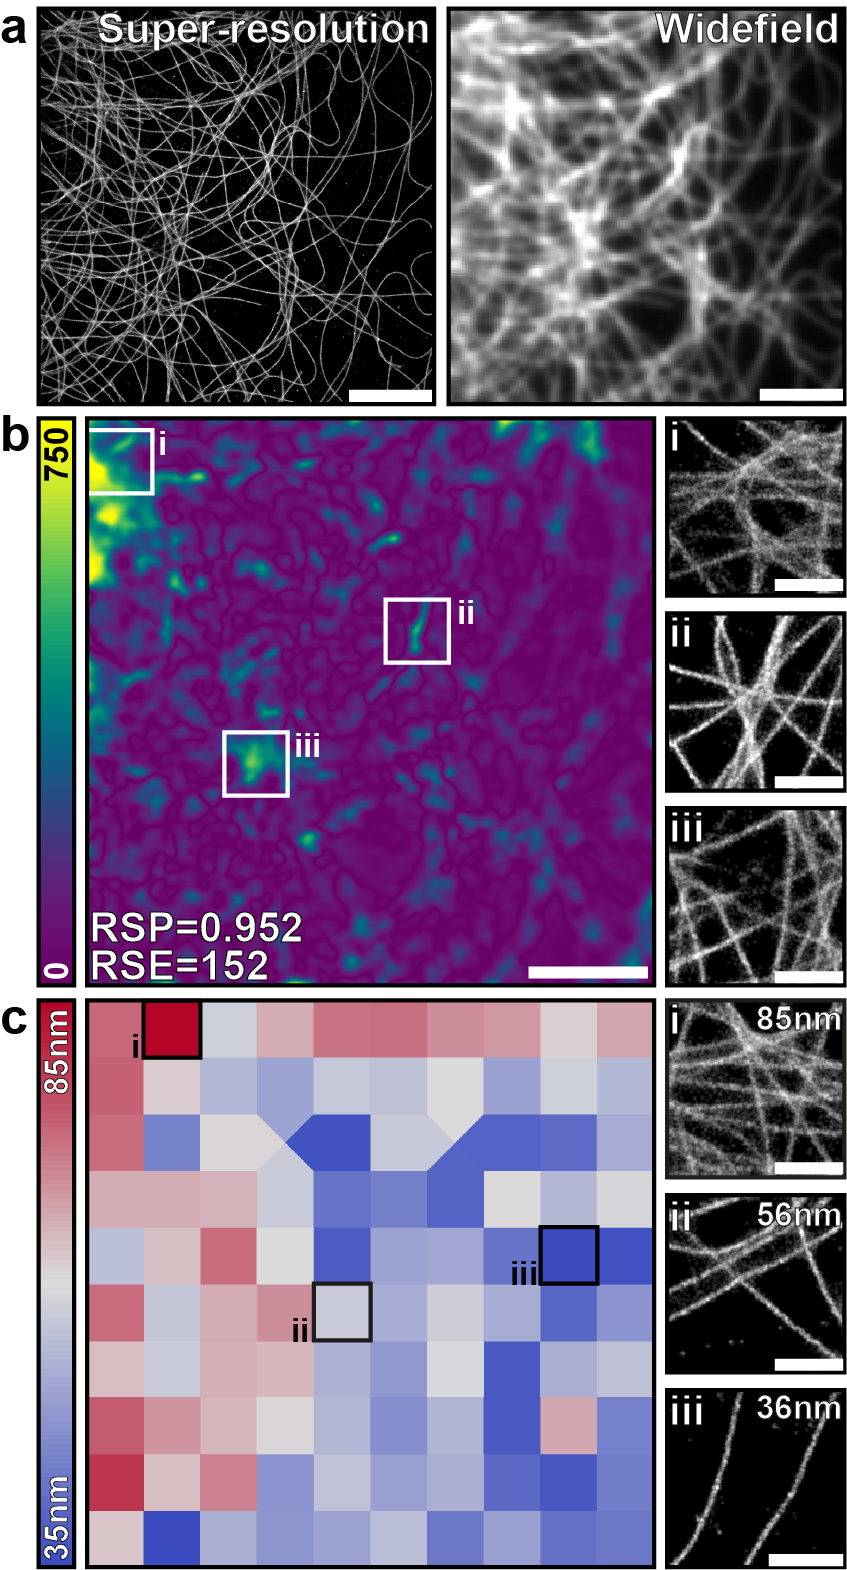
\includegraphics{Figures/FigureSQUIRREL_v2.png}
    \caption{\textbf{Quality assessment and resolution mapping with NanoJ-SQUIRREL.} \textbf{a)} A super-resolution rendering (left) and acquired widefield image (right) of fixed microtubules labelled with Alexa Fluor-647. \textbf{b)} Left: SQUIRREL error map highlighting discrepancies between the super-resolution and diffraction-limited images in (a). Right: Magnified insets of super-resolution rendering at indicated positions on error map. \textbf{c)} Left: SQUIRREL resolution map of the super-resolution image in (a). Right: Magnified insets of super-resolution rendering for indicated resolution blocks. Whole image scale bars = 5\micro m, inset scale bars = 1\micro m}
    \label{fig:SQUIRREL}
 \end{figure}
 %TC:endignore

\subsection*{NanoJ-SQUIRREL: Estimating Image Resolution}
The purpose of SRM is to resolve finer structural detail than is achievable with conventional diffraction-limited microscopy. It is therefore useful to have an objective measurement of resolution within a super-resolution image, for example to enable comparisons with known structure sizes from electron microscopy. The current standard for measuring image resolution in SMLM images is Fourier Ring Correlation (FRC) \cite{nieuwenhuizen2013measuring}. This method involves comparing two independently acquired super-resolution images of the same field-of-view so that they only differ by their noise component. For SMLM datasets the two SRM images are usually obtained by splitting localisations from odd and even frames. The correlation between these two images is measured at different frequencies in Fourier space; the frequency at which this correlation drops below a set threshold indicates the resolution of the image.

 FRC has been previously implemented in ImageJ \cite{nieuwenhuizen2013measuring}, but only gives a single resolution measurement for the entire field of view. However, resolution is not necessarily homogeneous across a super-resolution image. This is particularly true for SMLM methods as localisation accuracy depends strongly on labelling density and laser illumination intensity, which can both vary considerably within a single field of view. Furthermore, FRC can generate biased measurements for certain fluorophore distributions such as point-like patterns. Therefore an additional feature of the NanoJ-SQUIRREL plugin is local mapping of FRC resolution across an image. To do this, the user provides an image stack comprising two independent renderings of the same dataset (e.g. through the odd/even frames splitting as described above). The image is then split into equal-sized blocks and FRC analysis is run locally on each block. For blocks where there is insufficient correlation to generate an FRC resolution value, a resolution value is interpolated from neighbouring blocks. Fig. \ref{fig:SQUIRREL}c shows the FRC map obtained from the SRM image shown in (a). This map highlights that the resolution in this image varies between 85 and 36 nm.

It is important to note that high resolution (that is, a low FRC value) does not imply that the super-resolution image has depicted structures correctly; it only means that there is low variation in the locations of the fluorophores between the two rendered images. Therefore it is advisable to use the error mapping functionality within NanoJ-SQUIRREL alongside FRC mapping in order to obtain a more complete perspective on super-resolution image quality.

\subsection*{NanoJ-VirusMapper: Structural Mapping and Modelling}
 As part of the NanoJ framework, we include a unique single-particle analysis (SPA) tool called NanoJ-VirusMapper. It is the first open-source, freely available algorithm for unbiased, high-throughput SPA of fluorescence imaging and allows the structural modelling of viruses and other macro-molecular complexes \cite{gray2016virusmapper,gray2017open,gray2018nanoscale}. The principle of SPA is to image many identical copies of a structure, possibly in different orientations, align and combine them to build an averaged structural map of the underlying structure with high signal-to-noise ratio \cite{Szymborska2013,laine2015structural,lelek2012superresolution} . 
 
  \begin{figure}[!t]
    \centering
    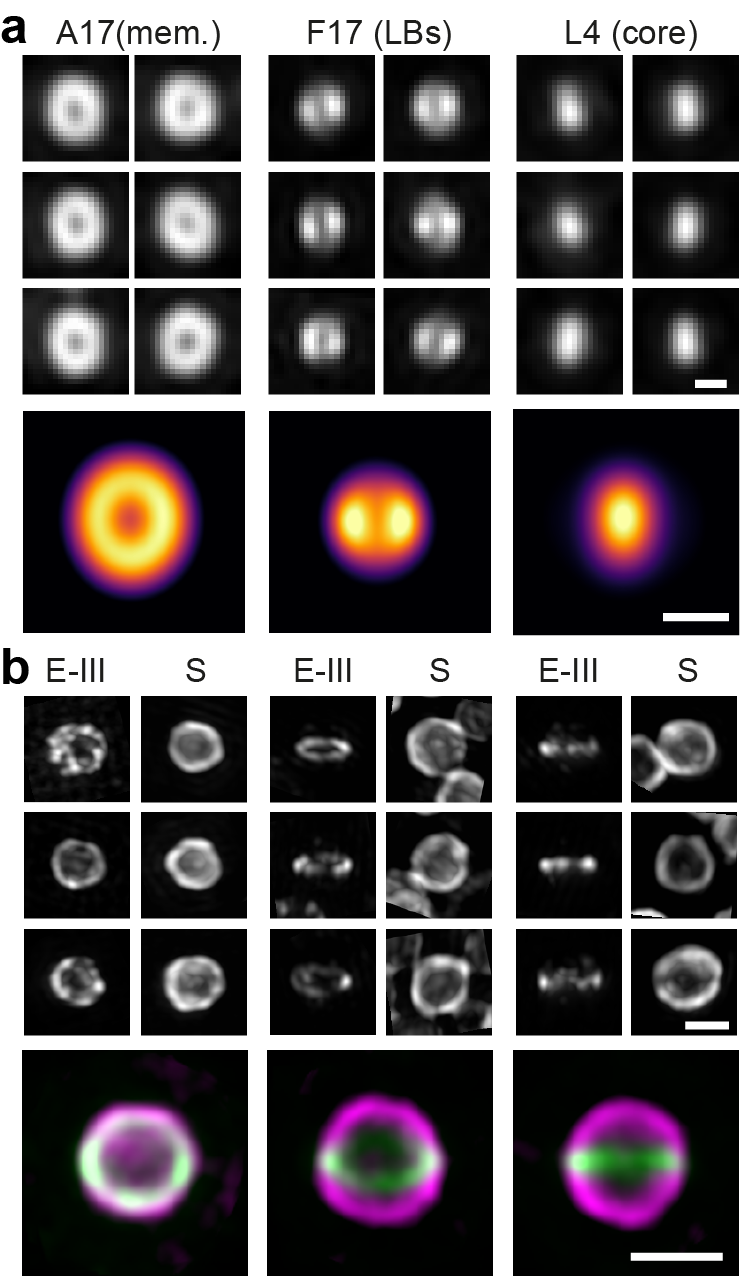
\includegraphics{Figures/NanoJ_VirusMapperFigure_v3.png}
    \caption{\textbf{Quantitative SPA-based modelling with NanoJ-VirusMapper.} \textbf{a)} Top: SIM images of individual vaccinia particles labelled for L4 (core), F17 (lateral body, LB) and A17 (membrane, mem.). Bottom: VirusMapper models of the three channels. Scale bars: 200nm. \textbf{b)} Top: SIM images of individual \emph{Sulfolobus} cells labelled for the S-layer (S) and ESCRT-III (E-III). Bottom: VirusMapper models of three different orientations of the cells. Scale bars: 1\micro m. }
    \label{fig:VirusMapper}
 \end{figure}

 The SPA implementation of VirusMapper facilitates automatic processing of multiple images to detect, segment, align, classify and average thousands of individual structures. Unlike other SPA applications it is entirely general, assuming no underlying symmetry or other properties of the imaged structure. Here, we illustrate this with models of three distinct vaccinia virus \cite{FieldsVirology2013} substructures: core, lateral bodies (LBs) and membrane. All three substructures were labelled on viral particles and imaged with Structured Illumination Microscopy (SIM) \cite{gustafsson2000surpassing} (Fig. \ref{fig:VirusMapper}a, top). The SIM images from each channel were then independently processed with VirusMapper to create models of the three components of the virus (Fig. \ref{fig:VirusMapper}a, bottom). Additionally, a key advantage of VirusMapper is that models from different channels can be aligned to each other.

 VirusMapper is capable of identifying and analysing different orientations of the same structure. Here, we highlight this capability on a study of the division ring in the archaeal type strain \emph{Sulfolobus acidocaldarius} DSM639 (Fig. \ref{fig:VirusMapper}b). \emph{Sulfolobus} cells were labelled for their outer S-layer and the division ring as marked by ESCRT-III proteins. The models from both channels were built from aligning the S-layer channel.

 VirusMapper has been demonstrated with SIM and stimulated emission depletion (STED) microscopy \cite{gray2016virusmapper} but is compatible with any fluorescence microscopy method, including SMLM.

\subsection*{NanoJ-Fluidics: Sample Liquid Exchange}

 NanoJ-Fluidics is a hardware and software framework for precise and accurate automated liquids exchange \cite{almada2018automating}. It was developed to enable automation of sample treatment and labelling of live or fixed cells directly on the microscope stage \cite{almada2018automating, dix2018role}. The NanoJ-Fluidics hardware component is composed of customisable, low-cost and robust LEGO® syringe pumps and a liquid removal peristaltic pump, both controlled by simple Arduino® electronics. It is compatible with off-the-shelf imaging chambers, without the need for any microfabrication. Its control software (the NanoJ-Fluidics module) is ImageJ-based and can be fully integrated with microscopy acquisition software. We have demonstrated the applicability of NanoJ-Fluidics in multiple experimental contexts, including \textit{in-situ} correlative live-to-fixed super-resolution imaging, multimodal super-resolution imaging and event-driven fixation \cite{almada2018automating}. The approach can also be easily extended to protocol optimization (e.g. titrating antibody concentrations or adjusting imaging buffer composition) or liquid exchange protocols integrated with the imaging (e.g. drug delivery or automated event-driven fixation).

 Here we demonstrate NanoJ-Fluidics by acquiring a high-quality multicolour SMLM dataset, where STORM and DNA-PAINT \cite{jungmann2014multiplexed} imaging strategies are combined into a single workflow (Fig. \ref{fig:PAINT}a). This approach is particularly suited to multi-target imaging \cite{dempsey2011evaluation}, which is difficult to achieve with standard sample preparation techniques due to the low number of suitable fluorophores available for SMLM microscopy. With NanoJ-Fluidics we can seamlessly perform all labelling steps in an automated and reliable manner directly on the microscope stage. We showcase this using a 4-channel acquisition of actin with STORM and mitochondria, vimentin and clathrin with DNA-PAINT (Fig. \ref{fig:PAINT}b). 

 NanoJ-Fluidics' highly customizable nature has already spawned several alternative designs from the community (\href{https://github.com/HenriquesLab/NanoJ-Fluidics/wiki}{https://github.com/HenriquesLab/NanoJ-Fluidics/wiki}), which are in constant development. NanoJ-Fluidics makes imaging protocol automation readily available to researchers, hence improving not only the reliability and repeatability of the protocols, but also the range of protocols that are achievable.  

 %TC:ignore
 \begin{figure}[!t]
    \centering
    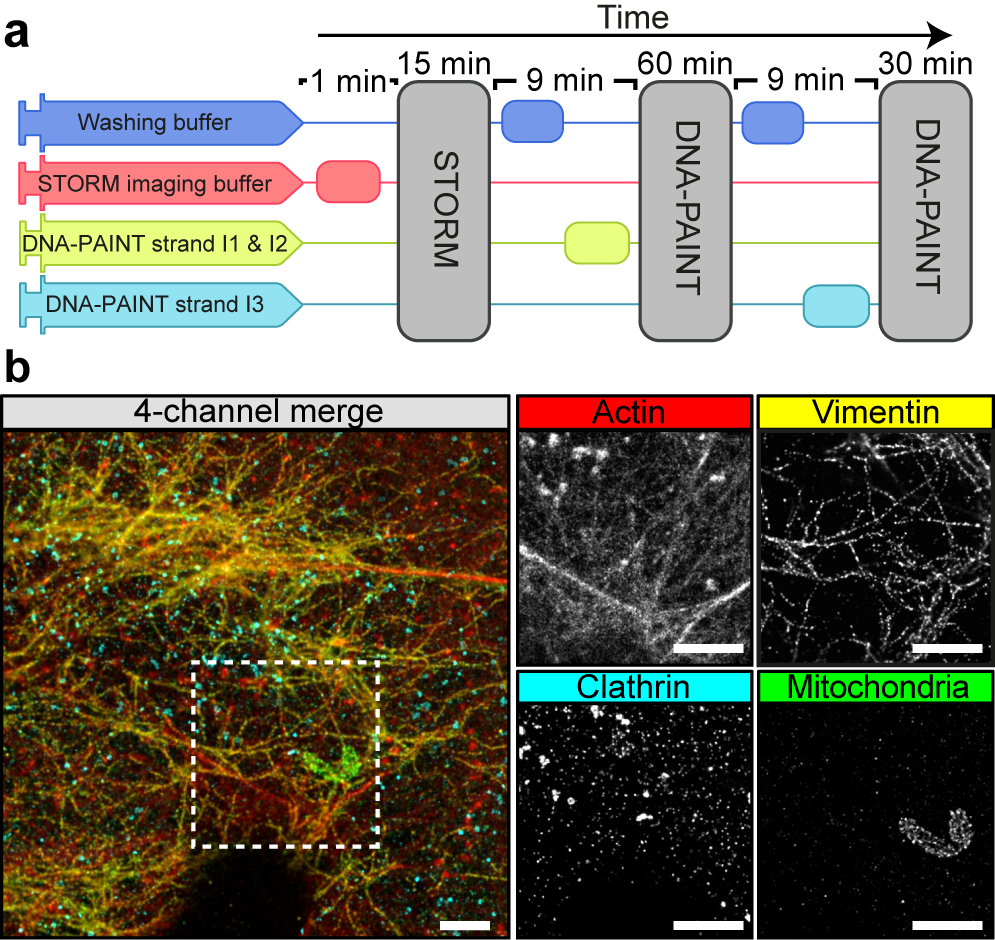
\includegraphics{Figures/FigurePumpy_v4.png}
    \caption{\textbf{Automated DNA-PAINT and STORM imaging.} \textbf{a)} NanoJ-Fluidics workflow used for multi-color STORM and DNA-PAINT imaging. \textbf{b)} Left: 4-channel merge of STORM and DNA-PAINT with actin (red), vimentin (yellow), clathrin (cyan) and mitochondria (green). Right: Single-channel images from the inset. Scale bars: 2 \textmu{}m.}
    \label{fig:PAINT}
 \end{figure}
 %TC:endignore

\subsection*{Discussion and Future Perspectives}
 The NanoJ framework provides a unique and comprehensive set of tools to support fluorescence imaging, from data acquisition and protocol optimisation to structural quantification. It offers powerful and user-friendly solutions to common pitfalls of image analysis such as drift correction and channel registration (NanoJ-Core). It extends the tools available for SRM to expert and novice users alike. It aligns with the general aim of the community to extend SRM to live-cell applications, offering the first open-source analytical approach for live-cell SRM imaging using any modern fluorescence microscope (NanoJ-SRRF). It Offers a way to correlate dynamic live-cell data with high-resolution fixed-cell data in an automated and highly reproducible manner (NanoJ-Fluidics). It Provides an analytical tool for the generation of accurate, high-content, molecular specific models and detection of nanoscale changes in biological architectures (NanoJ-VirusMapper). Finally, the NanoJ framework provides tools to quantitatively assess SRM image quality, by using spatially-varying FRC resolution maps, error (artefact) mapping, and image quality metrics (NanoJ-SQUIRREL). This aims to improve standards in assessing and reporting microscopy data. 
 The NanoJ framework allows users to access user-friendly yet robust analytical tools in tandem with new approaches to perform live-cell SRM experiments. A typical SRM live-cell imaging experiment using the NanoJ framework would entail acquiring a SRRF compatible raw data set in any modern fluorescence microscope; performing drift correction and channel registration; followed by SRRF analysis for SRM image reconstruction; and finally, quality checking using SQUIRREL. A pipeline that can be used for any biological question, seamlessly repeated for imaging protocol optimisation and complemented and expanded taking advantage of NanoJ-Fluidics and/or NanoJ-VirusMapper. The NanoJ-enabled scientific pipeline allows any user, regardless of the experience level, to seamlessly obtain SRM quantitative data of the highest scientific quality. 
 The NanoJ framework  was developed to facilitate access and expand the options of research groups using fluorescence microscopy. Hence, speed, reliability, performance and cross-compatibility are of paramount importance. In this context, NanoJ has been designed for high-performance image analysis, using GPU computing, ensuring the quick processing of large data volumes \cite{herbert2012single,pereira2015high,almada2015palm,beghin2017localization,douglass2016super}. Further, NanoJ' modular nature, open-source nature and its integration within ImageJ allow it to be used in conjunction with other analysis software packages \cite{sage2018super,weigert2017content,henriques2010quickpalm, laine2018milesim}. We are continuously supporting, adapting and expanding the framework to include new approaches. 
 
 NanoJ will set the standard of useful, open-source, high performance methods for the whole microscopy community.
 
\subsection*{Software and Hardware Availability}
 NanoJ follows open-source software and hardware standards. Each of its modules can be installed by enabling the corresponding code repository in Fiji or by following the instructions on the corresponding websites:
 \small
 \begin{itemize}
  \item \href{https://github.com/HenriquesLab/NanoJ-Core}{https://github.com/HenriquesLab/NanoJ-Core}
  \item \href{https://github.com/HenriquesLab/NanoJ-SRRF}{https://github.com/HenriquesLab/NanoJ-SRRF}
  \item \href{https://bitbucket.org/rhenriqueslab/nanoj-squirrel}{https://bitbucket.org/rhenriqueslab/NanoJ-SQUIRREL}
  \item \href{https://bitbucket.org/rhenriqueslab/NanoJ-VirusMapper}{https://bitbucket.org/rhenriqueslab/NanoJ-VirusMapper}
  \item \href{https://github.com/HenriquesLab/NanoJ-Fluidics}{https://github.com/HenriquesLab/NanoJ-Fluidics}
\end{itemize}

\begin{acknowledgements}
 We thank Prof. Ralf Jungmann at Max Planck Institute of Biochemistry Munich for reagents and advice. This work was funded by grants from the UK Biotechnology and Biological Sciences Research Council (BB/M022374/1; BB/P027431/1; BB/R000697/1; BB/S507532/1) (R.H., P.M.P. and R.F.L.), the UK Medical Research Council (MR/K015826/1) (R.H.), the Wellcome Trust (203276/Z/16/Z) (S.C., R.H and B.B.), Core funding to the MRC Laboratory for Molecular Cell Biology, University College London (MC\_UU12018/7) (J.M.), the European Research Council (649101—UbiProPox) (J.M.) and the Centre National de la Recherche Scientifique (CNRS ATIP-AVENIR program AO2016) (C.L.). N.G. and R.D.M.G funded by the Engineering and Physical Sciences Research Council (EP/L504889/1). P.A. was supported by a PhD fellowship from the UK’s Biotechnology and Biological Sciences Research Council. Research by B.B. was supported by UCL, Cancer Research UK (C1529/A17343), and MRC (MC\_CF12266). K.L.T. and G.T.R. supported by a 4-year MRC Research Studentship. D.A. is presently a Marie Curie fellow (Marie Sklodowska-Curie 750673).
\end{acknowledgements}

\begin{contributions}
 These contributions follow the Contributor Roles Taxonomy guidelines: \href{https://casrai.org/credit/}{https://casrai.org/credit/}.
 Conceptualization: K.L.T, R.F.L., N.G., R.D.M.G, P.A., D.A., G.T.R., B.B., J.M., C.L., P.M.P., S.C., R.H.;
 Data curation: K.L.T, R.F.L., R.D.M.G, G.T.R., J.M., C.L., P.M.P., S.C., R.H.;
 Formal analysis:  K.L.T, R.F.L., R.D.M.G, C.L., S.C.;
 Funding acquisition:  B.B., C.L., R.H.;
 Investigation: K.L.T, R.F.L., R.D.M.G, G.T.R., C.L., P.M.P., S.C.;
 Methodology: R.F.L., N.G., R.D.M.G, P.A., J.M., C.L., P.M.P., S.C., R.H.;
 Project administration: R.F.L., B.B., J.M., C.L., P.M.P., S.C., R.H.;
 Resources: K.L.T, R.D.M.G, D.A., G.T.R., A.L., B.B., J.M., C.L., P.M.P., S.C.;
 Software: R.F.L., N.G., R.D.M.G, P.A., C.L., P.M.P., S.C., R.H.;
 Supervision: R.F.L., A.L., B.B., J.M., C.L., P.M.P., S.C., R.H.;
 Validation: K.L.T, R.F.L., N.G., R.D.M.G, P.A., D.A., C.L., P.M.P., S.C.;
 Visualization:  K.L.T, R.F.L., R.D.M.G, D.A., C.L., P.M.P., S.C., R.H.;
 Writing – original draft: K.L.T, R.F.L., R.D.M.G, D.A., C.L., P.M.P., S.C., R.H.;
 Writing – review \& editing: all authors.

\end{contributions}

\begin{interests}
 The authors declare no competing financial interests.
\end{interests}

\section*{Bibliography}
\bibliographystyle{zHenriquesLab-StyleBib}
\bibliography{06_Bibliography_Clean}
